% !TeX spellcheck = en-US
% !TeX encoding = UTF-8
% !TeX root = ../thesis.tex

\chapter{Evaluation}
\label{ch:Evaluation}
% pages: 7.14-9.52

This section elaborates on the results of our experiments. As a proof of concept we aimed to show, that our architecture is able to learn rendezvous tasks with a more or less GNN Blocks (1). Then we compared training on a set of agents, while evaluating on a different amount of agents (2). Afterwards we showed the effect of different aggregation functions on training (3), and how multiple GNN hops can effect the result if the observation radius for the agent varies (4). 
%\begin{itemize}[noitemsep,nolistsep]
%    \item (1001-7-pursuit-multi-neighaggr)
%    \item (1001-8-directed-vs-undirected-graph)
%    \item (1001-9-value-nodewise-graphwise)
%\end{itemize} 
\par

Evalution of the results used different environments compared to training. While the agents trained on randomized starting positions, they were tested with fixed starting positions to allow comparable results. A similar setting was used for evader starting position in Pursuit environments. We considered the average reward per training step and the last reward per training step as performance metrics. The mean gave us a meaningfull metric for the progress of the RL algorithm, while the last reward had a more geometric importance for solving the tasks like Rendezvous.  \par

Unless mentioned otherwise, the following experimental settings were used:
Experiment settings that are generally true (overview, add Appendix for more details)
go through more of the settings for the environments used that are important, like agents have same starting position etc.
\begin{itemize}[noitemsep,nolistsep]
    \item Most plots show the standard error from the input data.
    \item The environment always used a torus setup (position is wrapped using modulo, no borders).
    \item Observations did not directly include the positions of agents or evaders which would trivialize the tasks.
    \item No observation culling was used: Each agent could see every other agent and evader.
    \item The agents used direct dynamics: Their actions directly influenced movement on the x- and y-Axis.
    \item Rewards and Observation were normalized using a running mean and std to improve learning.
    \item Used mean aggregation.
    \item Independet GNN-stack for the actor and critic, which used residual connections.
    \item In heterogeneous graphs we used concatenation of the edge-types not aggregation
\end{itemize} \par

During the evaluation of the experiments, we experienced unexpected hardware issues that caused a subset of our runs to crash. Due to time constraints we were not able to fully replicate the respective experiments. Note that we do not include these crashed runs in our evaluation, and that the resulting grid searches are thus partially incomplete. The general findings of this thesis remain unchanged. \par



\section{Proof of Concept}
\label{sec:Proof of Concept}
% >= 1.5 pages
This proof of concept experiment used rendezvous. We wanted to show in a simpler environment that our architecture works in general. Furthermore we wanted to investigate if multiple number of hops can already have an impact on learning for rendezvous without any observation culling. We choose to use 10 agents that have 24 timesteps to meet each other in a torus-world of size 12. For these runs we used latent-dimension in the range of 8 to 64 and 1 to 4 number of hops. The last reward of a given iteration tells us if the agents were able to meet up in the alotted time and therefore we choose that as a comparison.

\begin{figure}[htp]
    \centering
    \subfigure[number of hops]{\label{fig:proof_of_concept_rendezvous_1}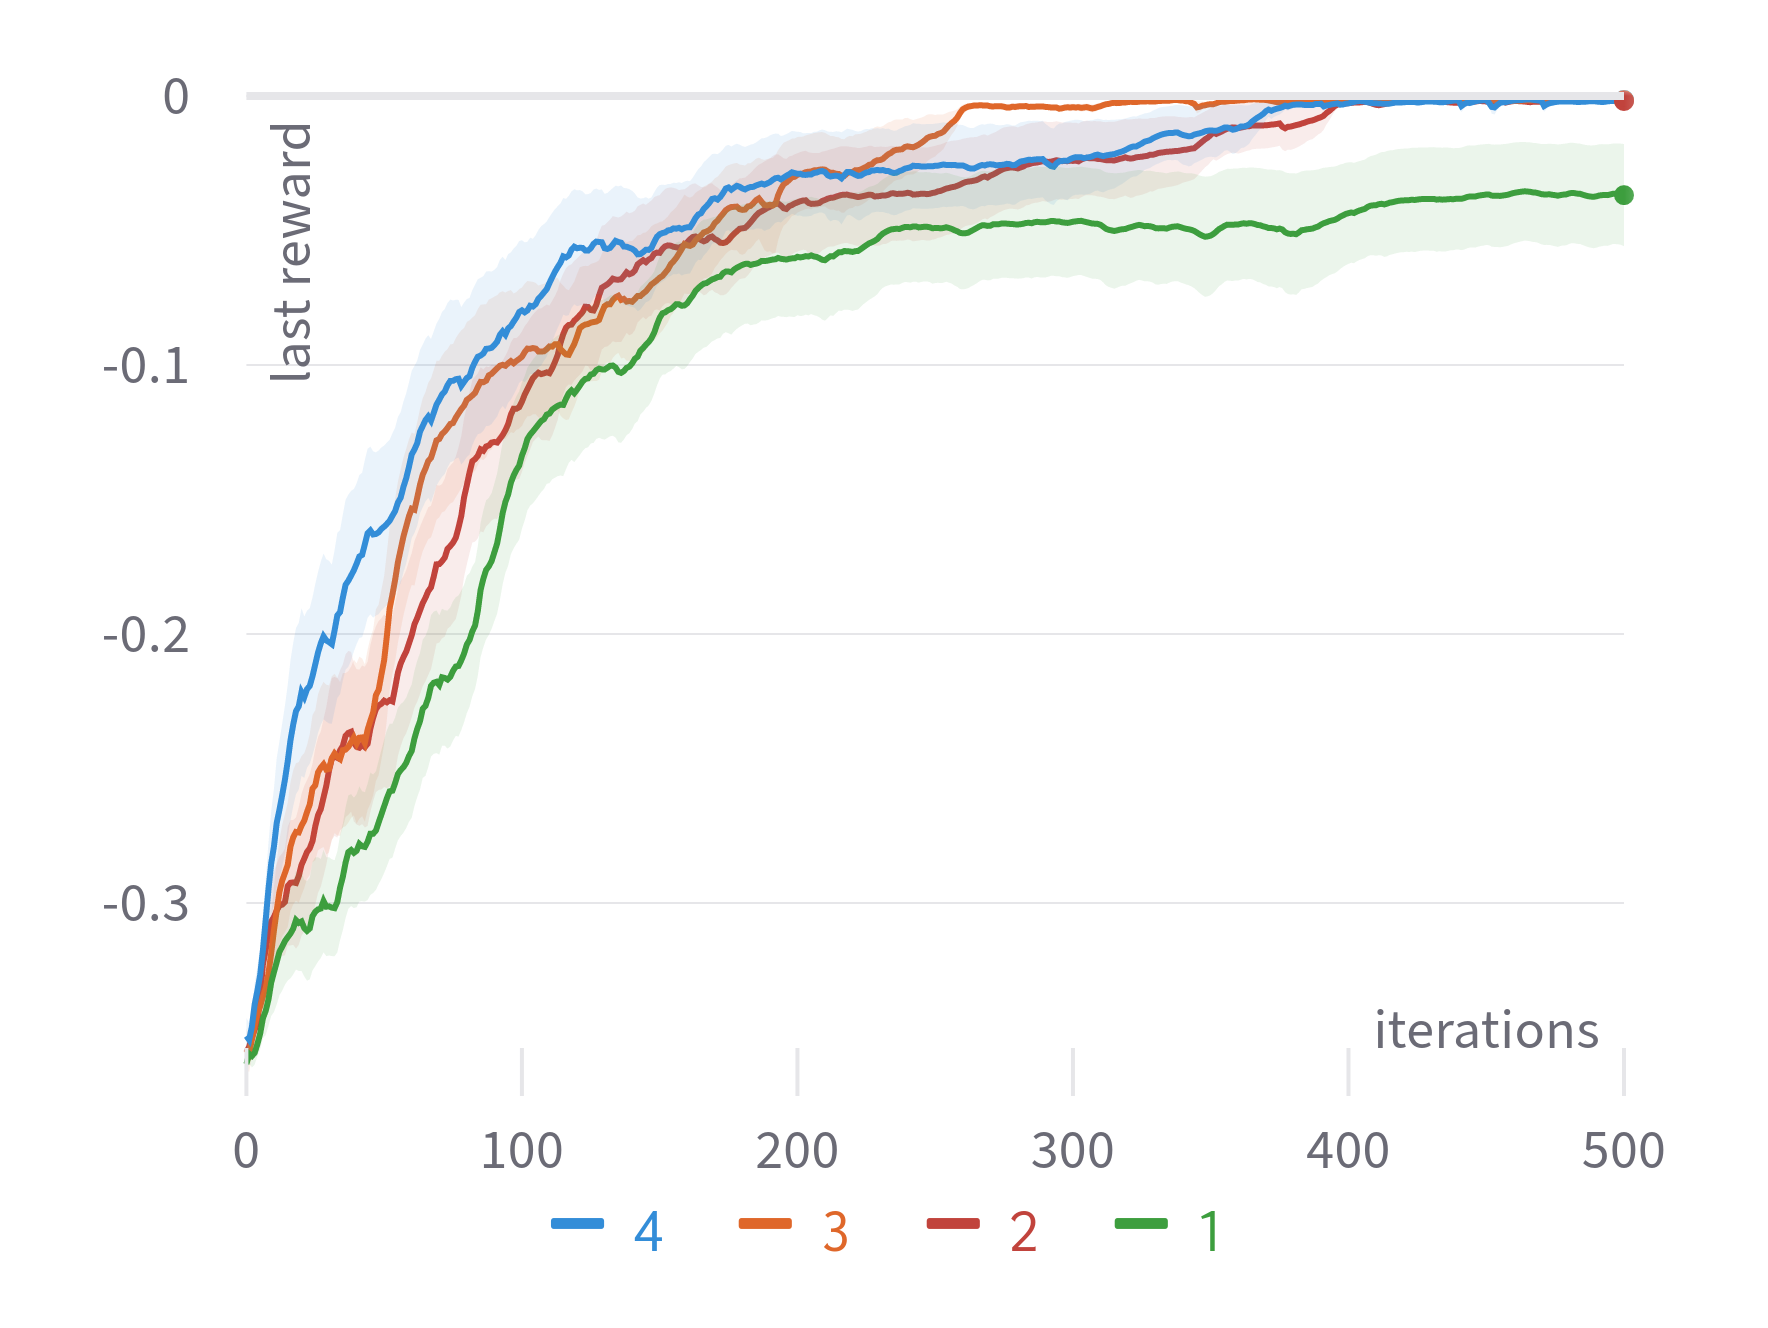
\includegraphics[width=0.49\textwidth]{figures/proof_of_concept_rendezvous_1.png}}  
    \subfigure[latent dimension]{\label{fig:proof_of_concept_rendezvous_2}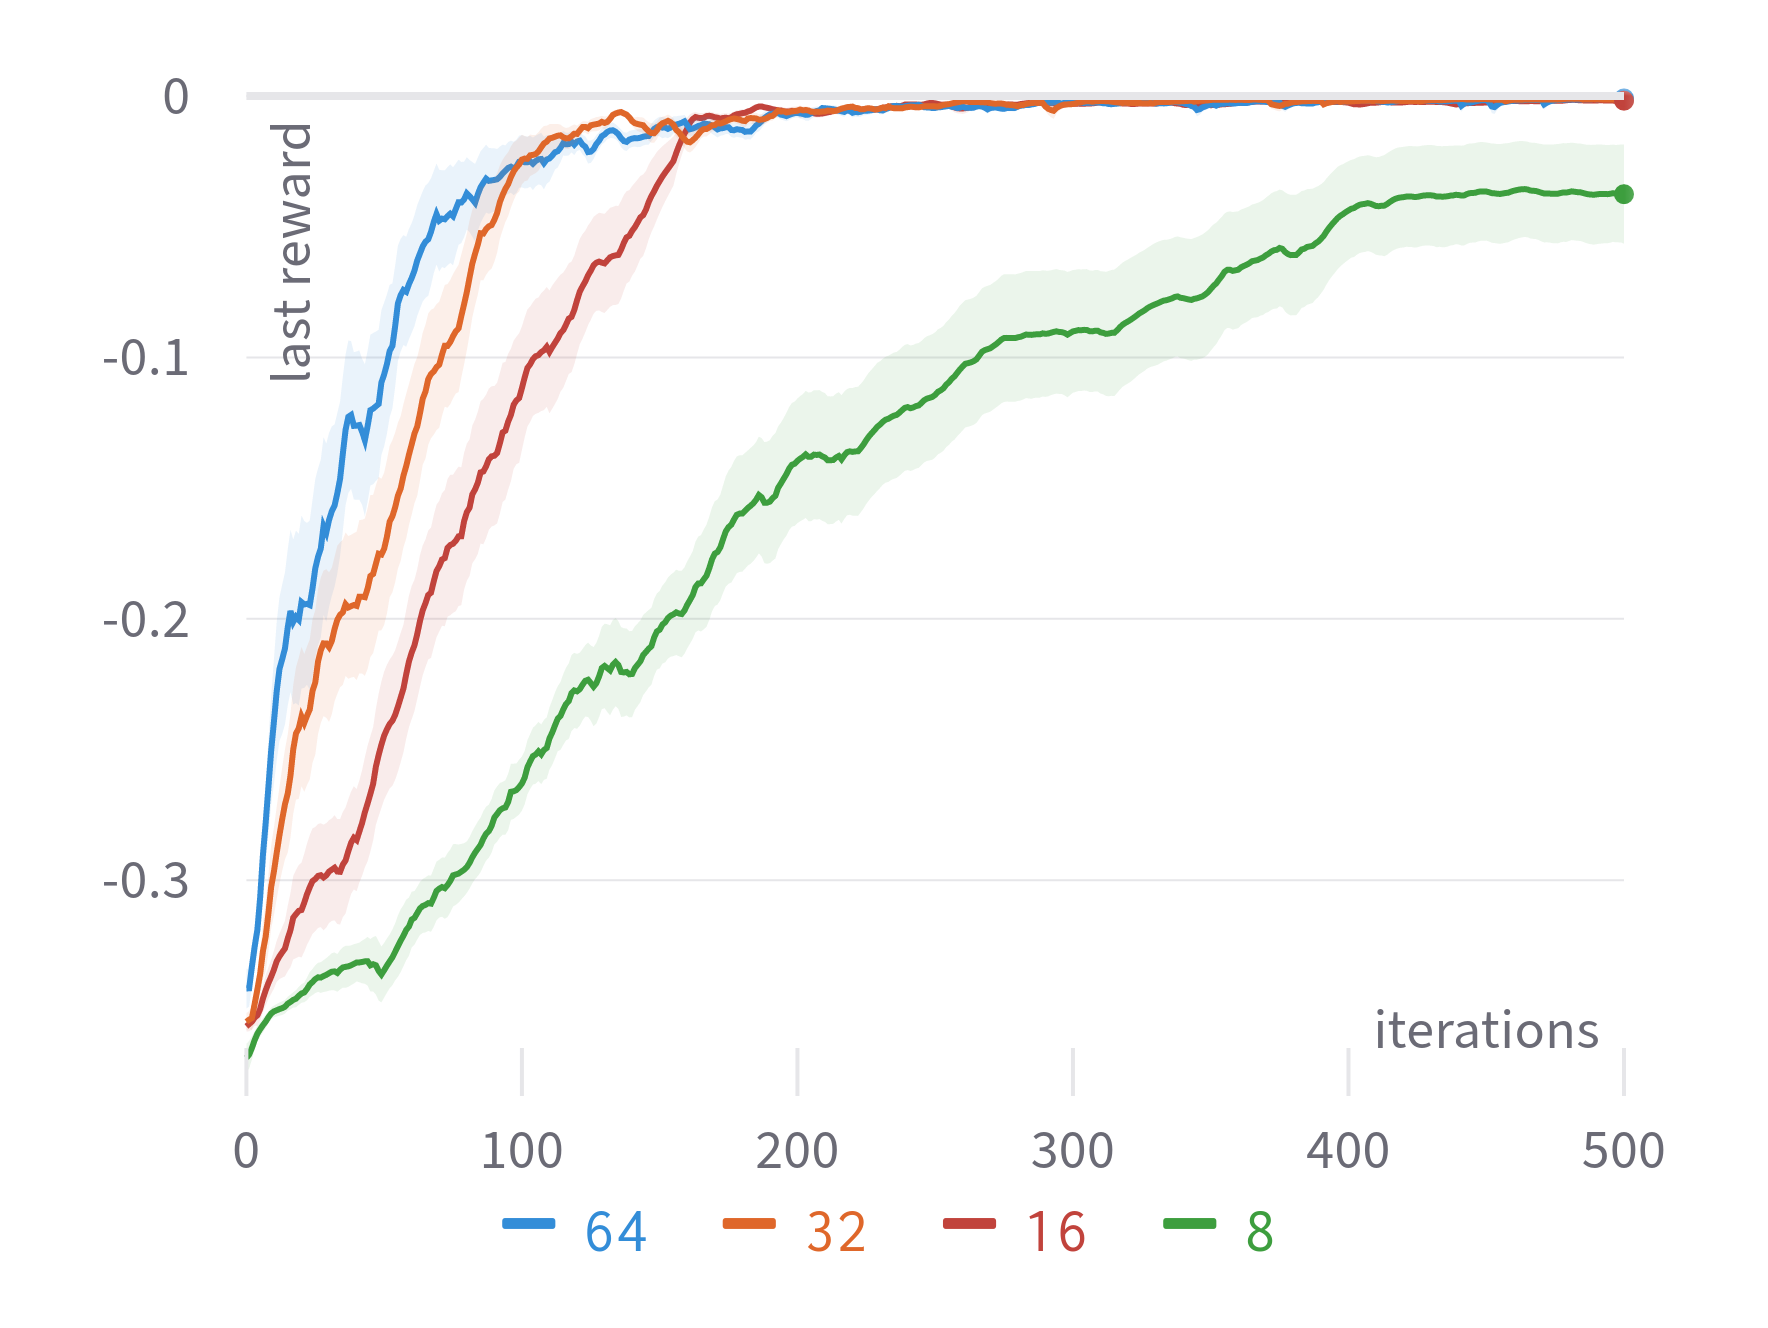
\includegraphics[width=0.49\textwidth]{figures/proof_of_concept_rendezvous_2.png}}  
    \hspace{1cm}                       
    \caption{Results of the Rendezvous task for different latent dimensions. The left side shows that more hops help in rendezvous, though the effect drops of sharply after 2-3 hops. }
    \label{fig:proof_of_concept_rendezvous}
\end{figure}

\Cref{fig:proof_of_concept_rendezvous} clearly shows that most of the training environments were able to successfully solve the task. With at least 2 hops, the task was solved after 200 to 350 iterations. The difference in Rendezvous for more than 2 hops is pretty noisy. In early iterations, performance is directly tied to more hops. But later the difference between 2-4 gets smaller. 4 Even struggles to optimize beyond a ceratin threshhold for a while. It is clear that the architecture is able effect the observation input more strongly, and learn faster. Each extra hop added roughly 13$\%$ to the time needed to learn, so the benefit is rather small. This was expected though for a rather simple task. If we look at the right site, we can see the effect of different latent dimension to the effectiveness of learning. Only a latent-dimension of 8 was not enough for the agents to meet up in the alotted time. It is clear that the architecture was not able to correctly represent and process observation data for 10 agents.\par

\begin{figure}[htp]
    \centering
    \subfigure[latent-dimension: 8]{\label{fig:proof_of_concept_rendezvous_ld8}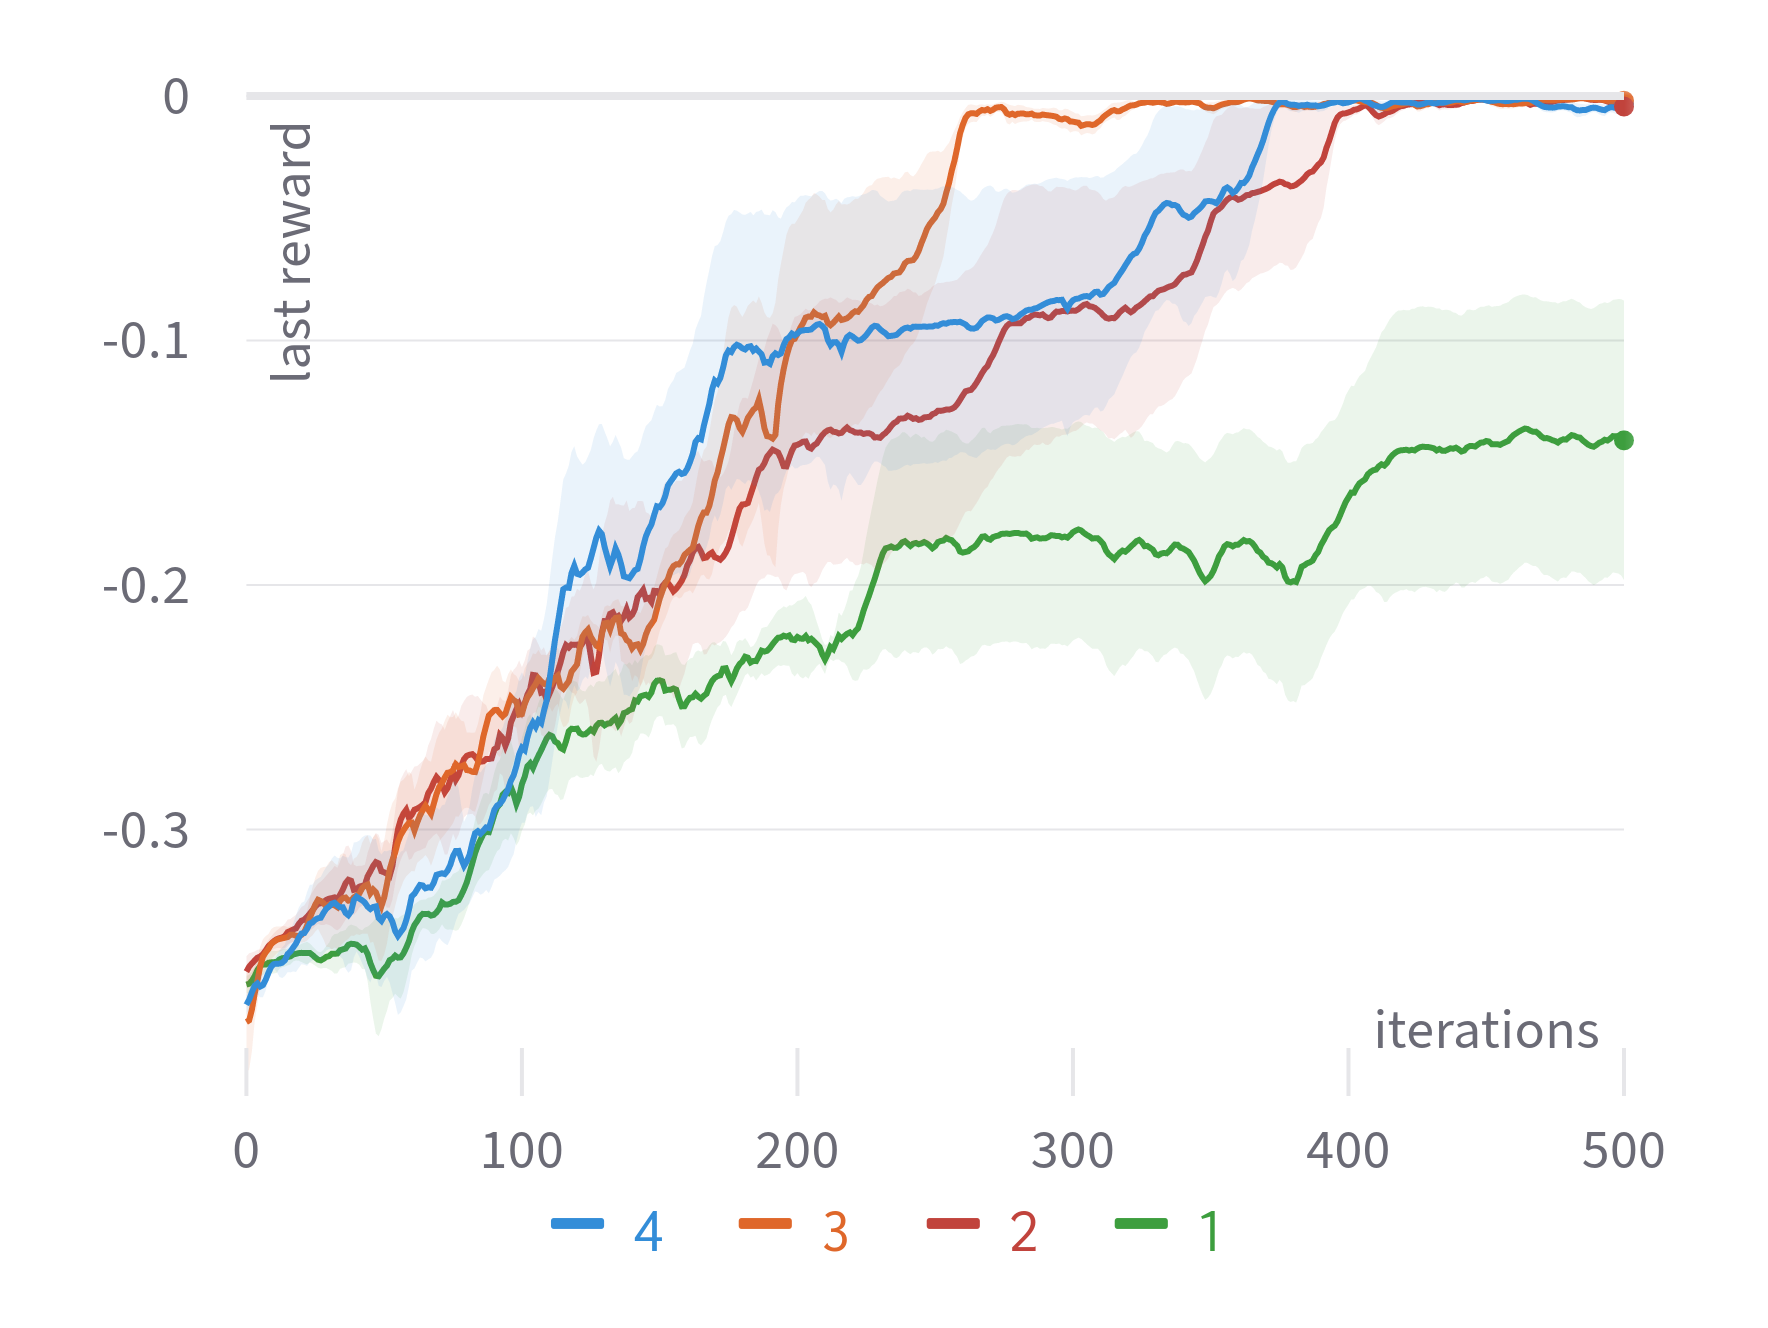
\includegraphics[width=0.49\textwidth]{figures/proof_of_concept_rendezvous_ld8.png}}  
    \subfigure[latent-dimension: 16]{\label{fig:proof_of_concept_rendezvous_ld16}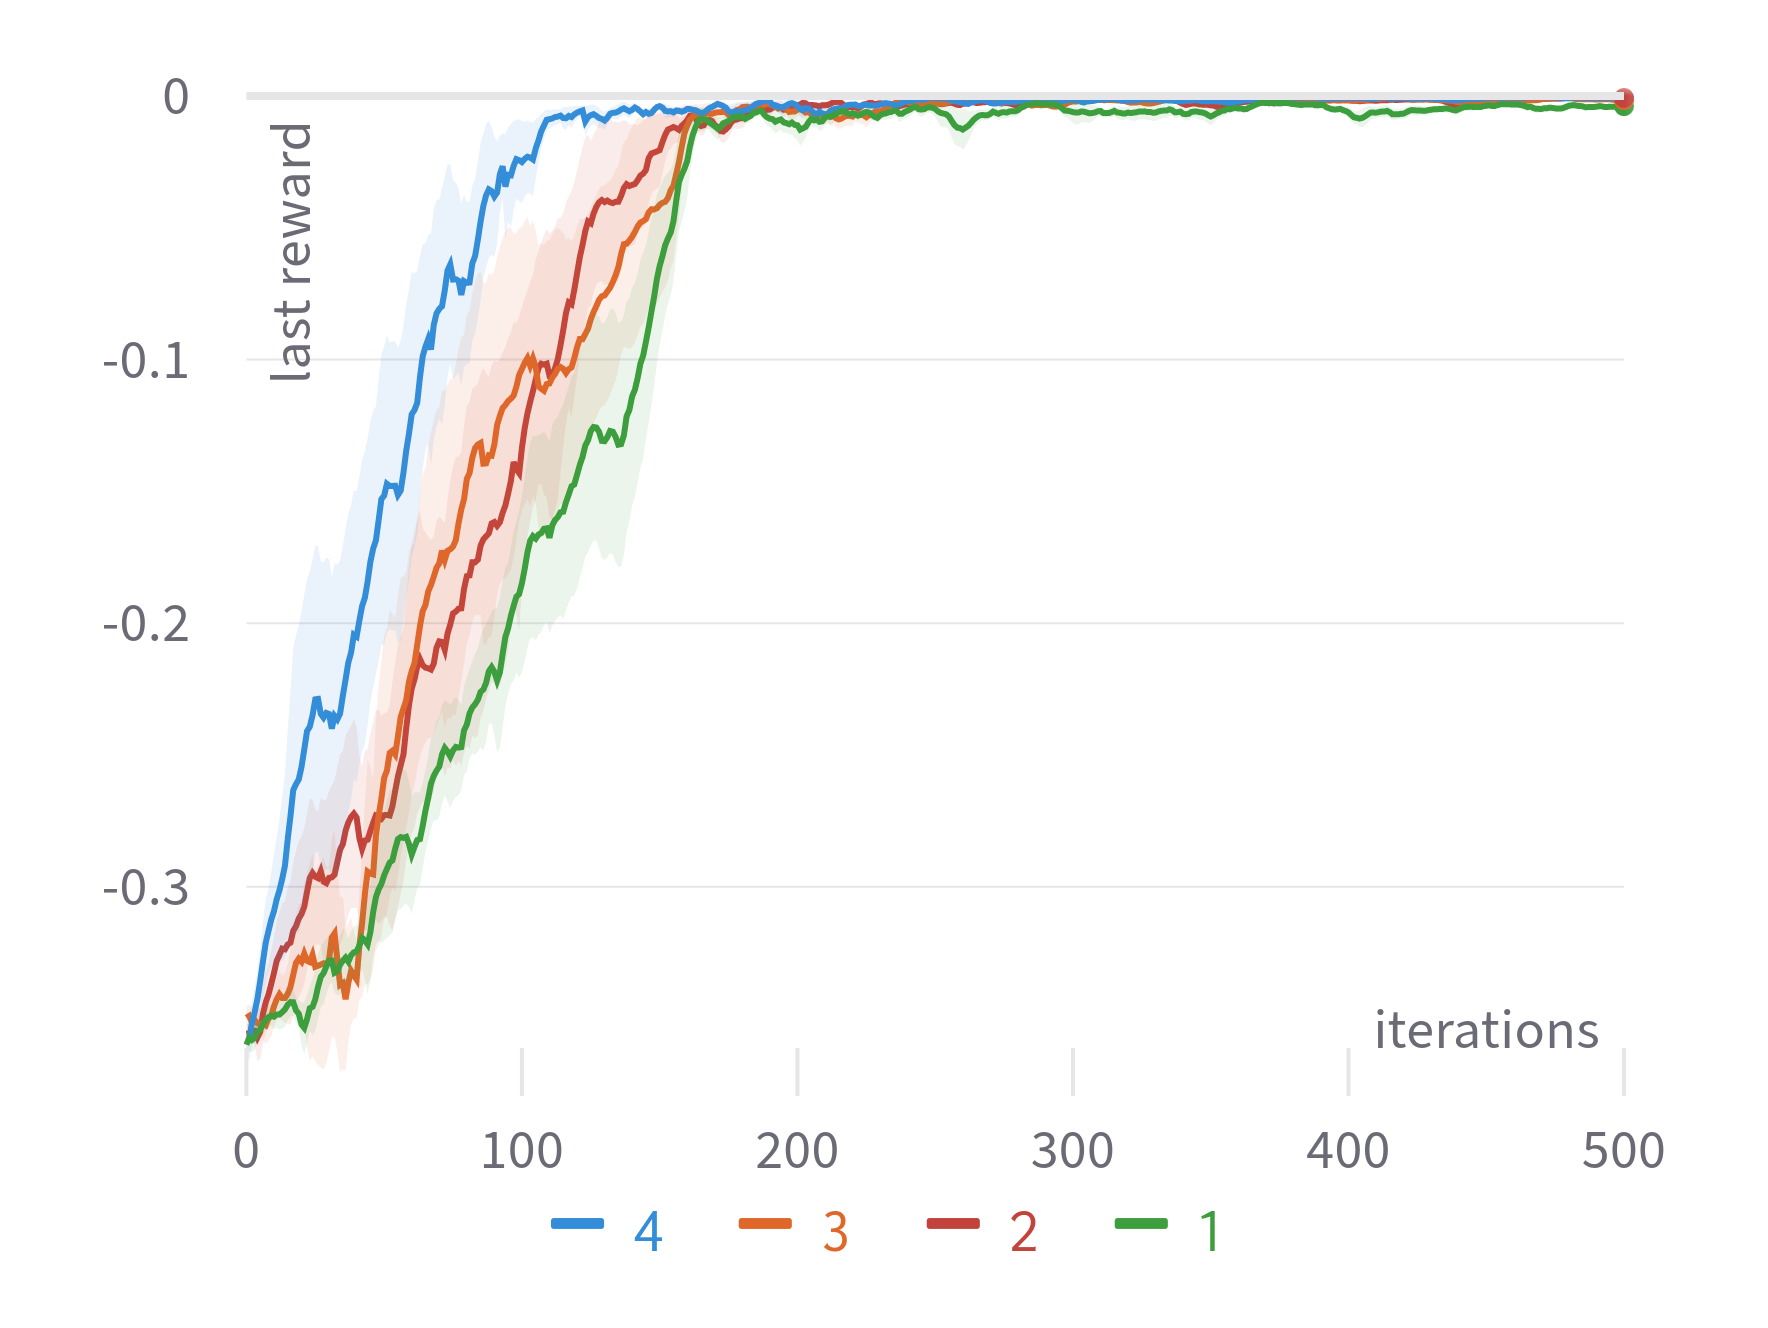
\includegraphics[width=0.49\textwidth]{figures/proof_of_concept_rendezvous_ld16.png}}  
    \hspace{1cm}                       
    \caption{When we filter for latent-dimension of 8, we can clearly see a larger gap between 2-4 hops and just 1 hop on the left side. For latent-dimension larger than 8, this different becomes smaller and more noisy.}
    \label{fig:proof_of_concept_rendezvous_ld}
\end{figure}

If we investigate the behavior for the different latent-dimensions, we can see a large difference in performance shown in \Cref{fig:proof_of_concept_rendezvous_ld}. Latent-dimensions 16 or more were able to solve the task easily. Here the gain of 4 hops is even stronger than comparing it to the general case. If we look at latent-dimension 8 it is clear that a single hop is a very strong outlier. The general performance is much worse, as it is not able to correctly represent the problem at hand. But the overall performance gain of 2 and more hops is much stronger. This shows in larger constraints the ability to process more of the observation data leads to a larger gain. Doubling the latent-dimensions roughly doubled the total time needed, much more than increasing the number of hops. This leads to the conclusion that more hops lead to larger runtime efficiency compared to higher latent dimension.


\section{Ablation}
\label{sec:Ablation}
% >= 1.5 pages
Which environments used and special setting, (grid)
\begin{itemize}[noitemsep,nolistsep]
    \item Environments: Rendezvous
    \item Environment: min-num-agent, max-num-agent (also for evaluation environment).
    \item Network: latent-dimension, num-blocks
\end{itemize}
Questions to answer: (what we wanted to show)
\begin{itemize}[noitemsep,nolistsep]
    \item How good is the GNN structure able to abstract to different amounts of agents?
    \item 
\end{itemize}
(Expected) Result:
\begin{itemize}[noitemsep,nolistsep]
    \item 
\end{itemize}



\section{Different Aggregation Functions}
\label{sec:Different Aggregation Functions}
% >= 1.5 pages
Which environments used and special setting, (grid)
\begin{itemize}[noitemsep,nolistsep]
    \item Environments: Dispersion
    \item Environment: reward-type
    \item Network: latent-dimension, num-blocks, aggregation-function
\end{itemize}
Questions to answer: (what we wanted to show)
\begin{itemize}[noitemsep,nolistsep]
    \item Does the architecture learn better/worse under different reward-functions in dispersion?
    \item How does number of hops help this?
\end{itemize}
(Expected) Result:
\begin{itemize}[noitemsep,nolistsep]
    \item 
\end{itemize}


\section{Under Observation Constraints}
\label{sec:Under Observation Constraints}
% >= 1.5 pages
Which environments used and special setting, (grid)
\begin{itemize}[noitemsep,nolistsep]
    \item Environments: Rendezvous, Pursuit-Multi
    \item Environment: Culling Methods: more culling vs less culling
    \item Network: num-blocks, latent-dimension
\end{itemize}
Questions to answer:  (what we wanted to show)
\begin{itemize}[noitemsep,nolistsep]
    \item Multi-Hops (multiple Layers) => Agents use Evader-Nodes to cache information/data.
    \item Effect of Multi-Hops on different levels of culling on more difficult tasks. Are they able to negate worse communication ranges? Compare policy on large communication, 1 layer vs. small communication, alot of layers. knn: num-layers: everyone can always communicate.
    \item What happens with really tight observation range?
    \item Pursuit-Multi: Strategy better then Robin? (are they able to create groups?).
    \item Describe the strategies in the different scenarios.
\end{itemize}
(Expected) Result:
\begin{itemize}[noitemsep,nolistsep]
    \item Harsher Culling => More Layers better. Can partially compensate. Still not the same information. Information about neighbors-neighbor still contains information about neighbor itself => it is influenced.
    \item policy on large communication, 1 layer > small communication, alot of layers. BUT may take longer?
    \item More Hops => Usually Better, but has limit. Complexer task => More Hops better (especially Pursuit-Multi).
    \item tight observation: at certain point it fails, even with alot of layers.
\end{itemize}



\section{Neighbor Aggregation Types}
\label{sec:Neighbor Aggregation Types}
Which environments used and special setting, (grid)
\begin{itemize}[noitemsep,nolistsep]
    \item Environments: Pursuit-Single, Pursuit-Multi
    \item Environment: Base-Pursuit-Multi with 3+ Hops?
    \item Network: latent-dimension, aggregation-function, neighbor-aggregation (aggr(aggr()) vs concat(aggr())), num-blocks
\end{itemize}
Questions to answer:
\begin{itemize}[noitemsep,nolistsep]
    \item Agents better/worse being able to distinguish themselves from evaders for concat(aggr())?
    \item How does this effect aggregation function for aggr(aggr()). Where do I get better performance?
    \item How is the effect of more/less hopps here?
\end{itemize}
(Expected) Result:
\begin{itemize}[noitemsep,nolistsep]
    \item concat(aggr()): worse iteration time, but easier to learn heterogeneous graphs.
    \item aggr(aggr()): probably mean aggregation, there are more features "preserved".
    \item num-hops: more hops should have more of an effect in concat(aggr()).
\end{itemize}



\section{Directed vs Undirected GNN}
\label{sec:Directed vs Undirected GNN}
Which environments used and special setting, (grid)
\begin{itemize}[noitemsep,nolistsep]
    \item Environments: Pursuit-Multi, Pursuit-Single
    \item Just add this to each of the other experiments (?)
    \item Environements: use-directed-graph.
    \item Network: num-blocks, latent-dimension, aggregation-function, neighbor-aggregation, value-function-scope
\end{itemize}
Questions to answer:
\begin{itemize}[noitemsep,nolistsep]
    \item what "learns" better or has better information propagation
\end{itemize}
(Expected) Result:
\begin{itemize}[noitemsep,nolistsep]
    \item 
\end{itemize}



\section{Node-wise vs Graph-wise Value-function}
\label{sec:Node-wise vs Graph-wise Value-function}
Which environments used and special setting, (grid)
\begin{itemize}[noitemsep,nolistsep]
    \item Environments: Rendezvous, Pursuit-Single
    \item Just add this to each of the other experiments (?)
    \item Environements: 
    \item Network: num-blocks, latent-dimension, aggregation-function, neighbor-aggregation, value-function-scope
\end{itemize}
Questions to answer:
\begin{itemize}[noitemsep,nolistsep]
    \item graph-wise: more "true" to the original Single agent RL algorithms. Should correlate better? But need to figure out themselves which agent is responsible for a reward.
    \item node-wise: better able to to gauge which agent was responsible for a given value or reward. 
\end{itemize}
(Expected) Result:
\begin{itemize}[noitemsep,nolistsep]
    \item 
\end{itemize}